% -*- program: xelatex -*-

\documentclass[12pt, t]{beamer}
%%% ------------------------------------------------------------------------
% packages
\usepackage{tikz}
\usetikzlibrary{shapes.geometric, arrows, positioning, shapes, backgrounds}
\usepackage{graphicx}
\usepackage{lmodern}
\usepackage{adjustbox}
% conditional (for figures)
\usepackage{etoolbox}

\usepackage{fontspec}
\usepackage{fontawesome}

\usepackage{subcaption} % side-by-side figures
\usepackage{hyperref}

\newtoggle{dark}

%%% ------------------------------------------------------------------------
% Theming (dark or white)
\usetheme{default}
\useoutertheme[subsection=false]{miniframes}

% move navigation to footer
\setbeamertemplate{headline}{}
\makeatletter
\setbeamertemplate{footline}
  {%
  \begin{beamercolorbox}{section in head/foot}
    \vskip2pt\insertnavigation{\paperwidth}\vskip5pt
  \end{beamercolorbox}%
  }
\makeatother


% no navigation bar
\beamertemplatenavigationsymbolsempty

% switch!
\toggletrue{dark}
% \togglefalse{dark}

\iftoggle{dark}{%
	% some colors
	\definecolor{foreground}{RGB}{255,255,255}
	\definecolor{background}{RGB}{24,24,24}
	\definecolor{title}{RGB}{127,185,220}
	\definecolor{gray}{RGB}{116,116,116}
	\definecolor{hilight}{RGB}{250, 108, 0}
	\setbeamercolor{section in head/foot}{fg = title}
	% set colors for titles, etc.
	\setbeamercolor{titlelike}{fg=title}
	\setbeamercolor{subtitle}{fg=title}
	\setbeamercolor{institute}{fg=gray}
	\setbeamercolor{normal text}{fg=foreground,bg=background}
	% % set colors for itemize
	\setbeamercolor{item}{fg=title} % color of bullets
	\setbeamercolor{subitem}{fg=gray}
	\setbeamercolor{itemize/enumerate subbody}{fg=gray}
}{
	% some colors
	\definecolor{foreground}{RGB}{0, 0, 0}
	\definecolor{background}{RGB}{255,255,255}
	\definecolor{title}{RGB}{107,174,214}
	\definecolor{gray}{RGB}{116,116,116}
	\definecolor{hilight}{RGB}{228, 97, 0}
	\setbeamercolor{section in head/foot}{fg = title}
	% set colors
	\setbeamercolor{titlelike}{fg=title}
	\setbeamercolor{subtitle}{fg=title}
	\setbeamercolor{institute}{fg=gray}
	\setbeamercolor{normal text}{fg=foreground,bg=background}
	% set colors for itemize
	\setbeamercolor{item}{fg=foreground} % color of bullets
	\setbeamercolor{subitem}{fg=gray}
	\setbeamercolor{itemize/enumerate subbody}{fg=gray}
}


%%% ------------------------------------------------------------------------
% Meta
\title{Statistical Ecotoxicology - Improving the utilization of data for ecological risk assessment}   
\author{Eduard Szöcs} 
\institute{Institute for Environmental Sciences, University of Koblenz-Landau}
\date{Landau, 22.09.2016}



%%% ------------------------------------------------------------------------
\begin{document}
\begin{frame}
\titlepage
\end{frame}


%%% -------------------------------
\section{Past} 
\subsection{}
\begin{frame}
\frametitle{My field of research is somewhere between...}
\center
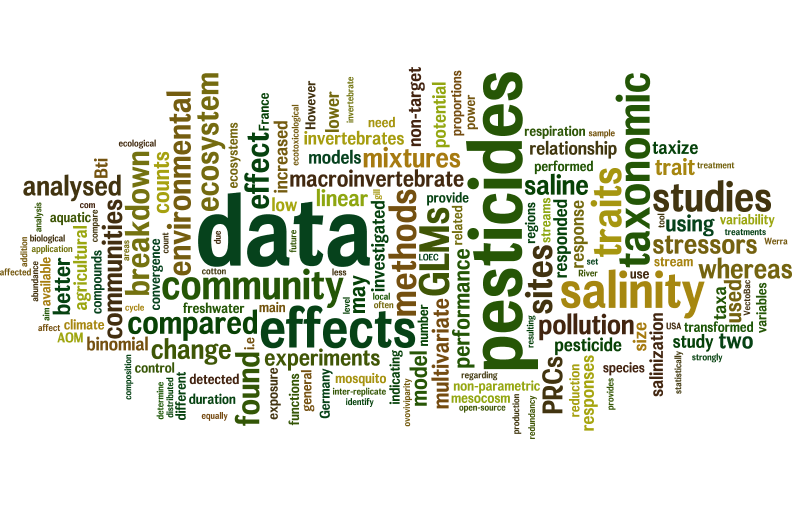
\includegraphics[width = 0.8\textwidth]{fit/wc_all.png} \\
\mbox{... Eco(-toxico)logy), Data Analysis & Programming}
\end{frame}


\begin{frame}
\frametitle{Statistical Power in current experimental designs in ecotoxicology is unacceptably low}

\end{frame}



\section{Present}
\subsection{}



\section{Future}
\subsection{}


\begin{frame}
\frametitle{}
\vspace{1em}
\begin{centering}
\Large \textcolor{title}{Data in Eco(toxico)logy} \\[1em]
Eduard Szöcs \\[0.3em]
\tiny \textcolor{gray}{Institute for Environmental Sciences, University of Koblenz-Landau} \\[5em]
\end{centering}
\normalsize
\textcolor{hilight}{\faLaptop}~~~\href{http://edild.github.io/}{http://edild.github.io/ }\\[.5em]
\textcolor{hilight}{\faTwitter}~~~\href{http://twitter.com/EduardSzoecs}{@EduardSzoecs} 	\\[0.5em]
\textcolor{hilight}{\faGift}~~~\href{https://github.com/edild/talk_work}{https://github.com/edild/talk\_work}\\[0.5em]
\textcolor{hilight}{\faEnvelope}~~~\href{mailto:szoecs@uni-landau.de}{szoecs@uni-landau.de} \\[.5em]
\hfill 
\includegraphics[width =.3\textwidth]{fig/Cc-by-nc_euro_icon.png} 
\end{frame}


\end{document}
